% ============================================== %

%%%%%%%%%%%%%%%%%%%%%%%%%%%%%%%%%%%%%%%%%%%%%%%%%%
%%%			  09 Trabalho Prático 09		   %%%
%%%%%%%%%%%%%%%%%%%%%%%%%%%%%%%%%%%%%%%%%%%%%%%%%%

% ============================================== %

\section{Trabalho Prático 09}

Encontrar o deslocamento $v$ no equilíbrio, considerando-se a medida de deformação de
Green e o algoritmo de Newton-Raphson na resolução. Adotar:

$$
\left\{\begin{array}{lcl}
	E   &=& 20.000\text{ kN/cm}^2 \\
	L   &=& 150\text{ cm} \\
	H   &=& 10\text{ cm} \\
	A_0 &=& 5\text{ cm}^2 \\
	P   &=& 20\text{ kN} \\
\end{array}\right.
$$

\begin{figure}[H]
	\centering
	\caption{Sistema estrutural do Trabalho Prático 09.}
	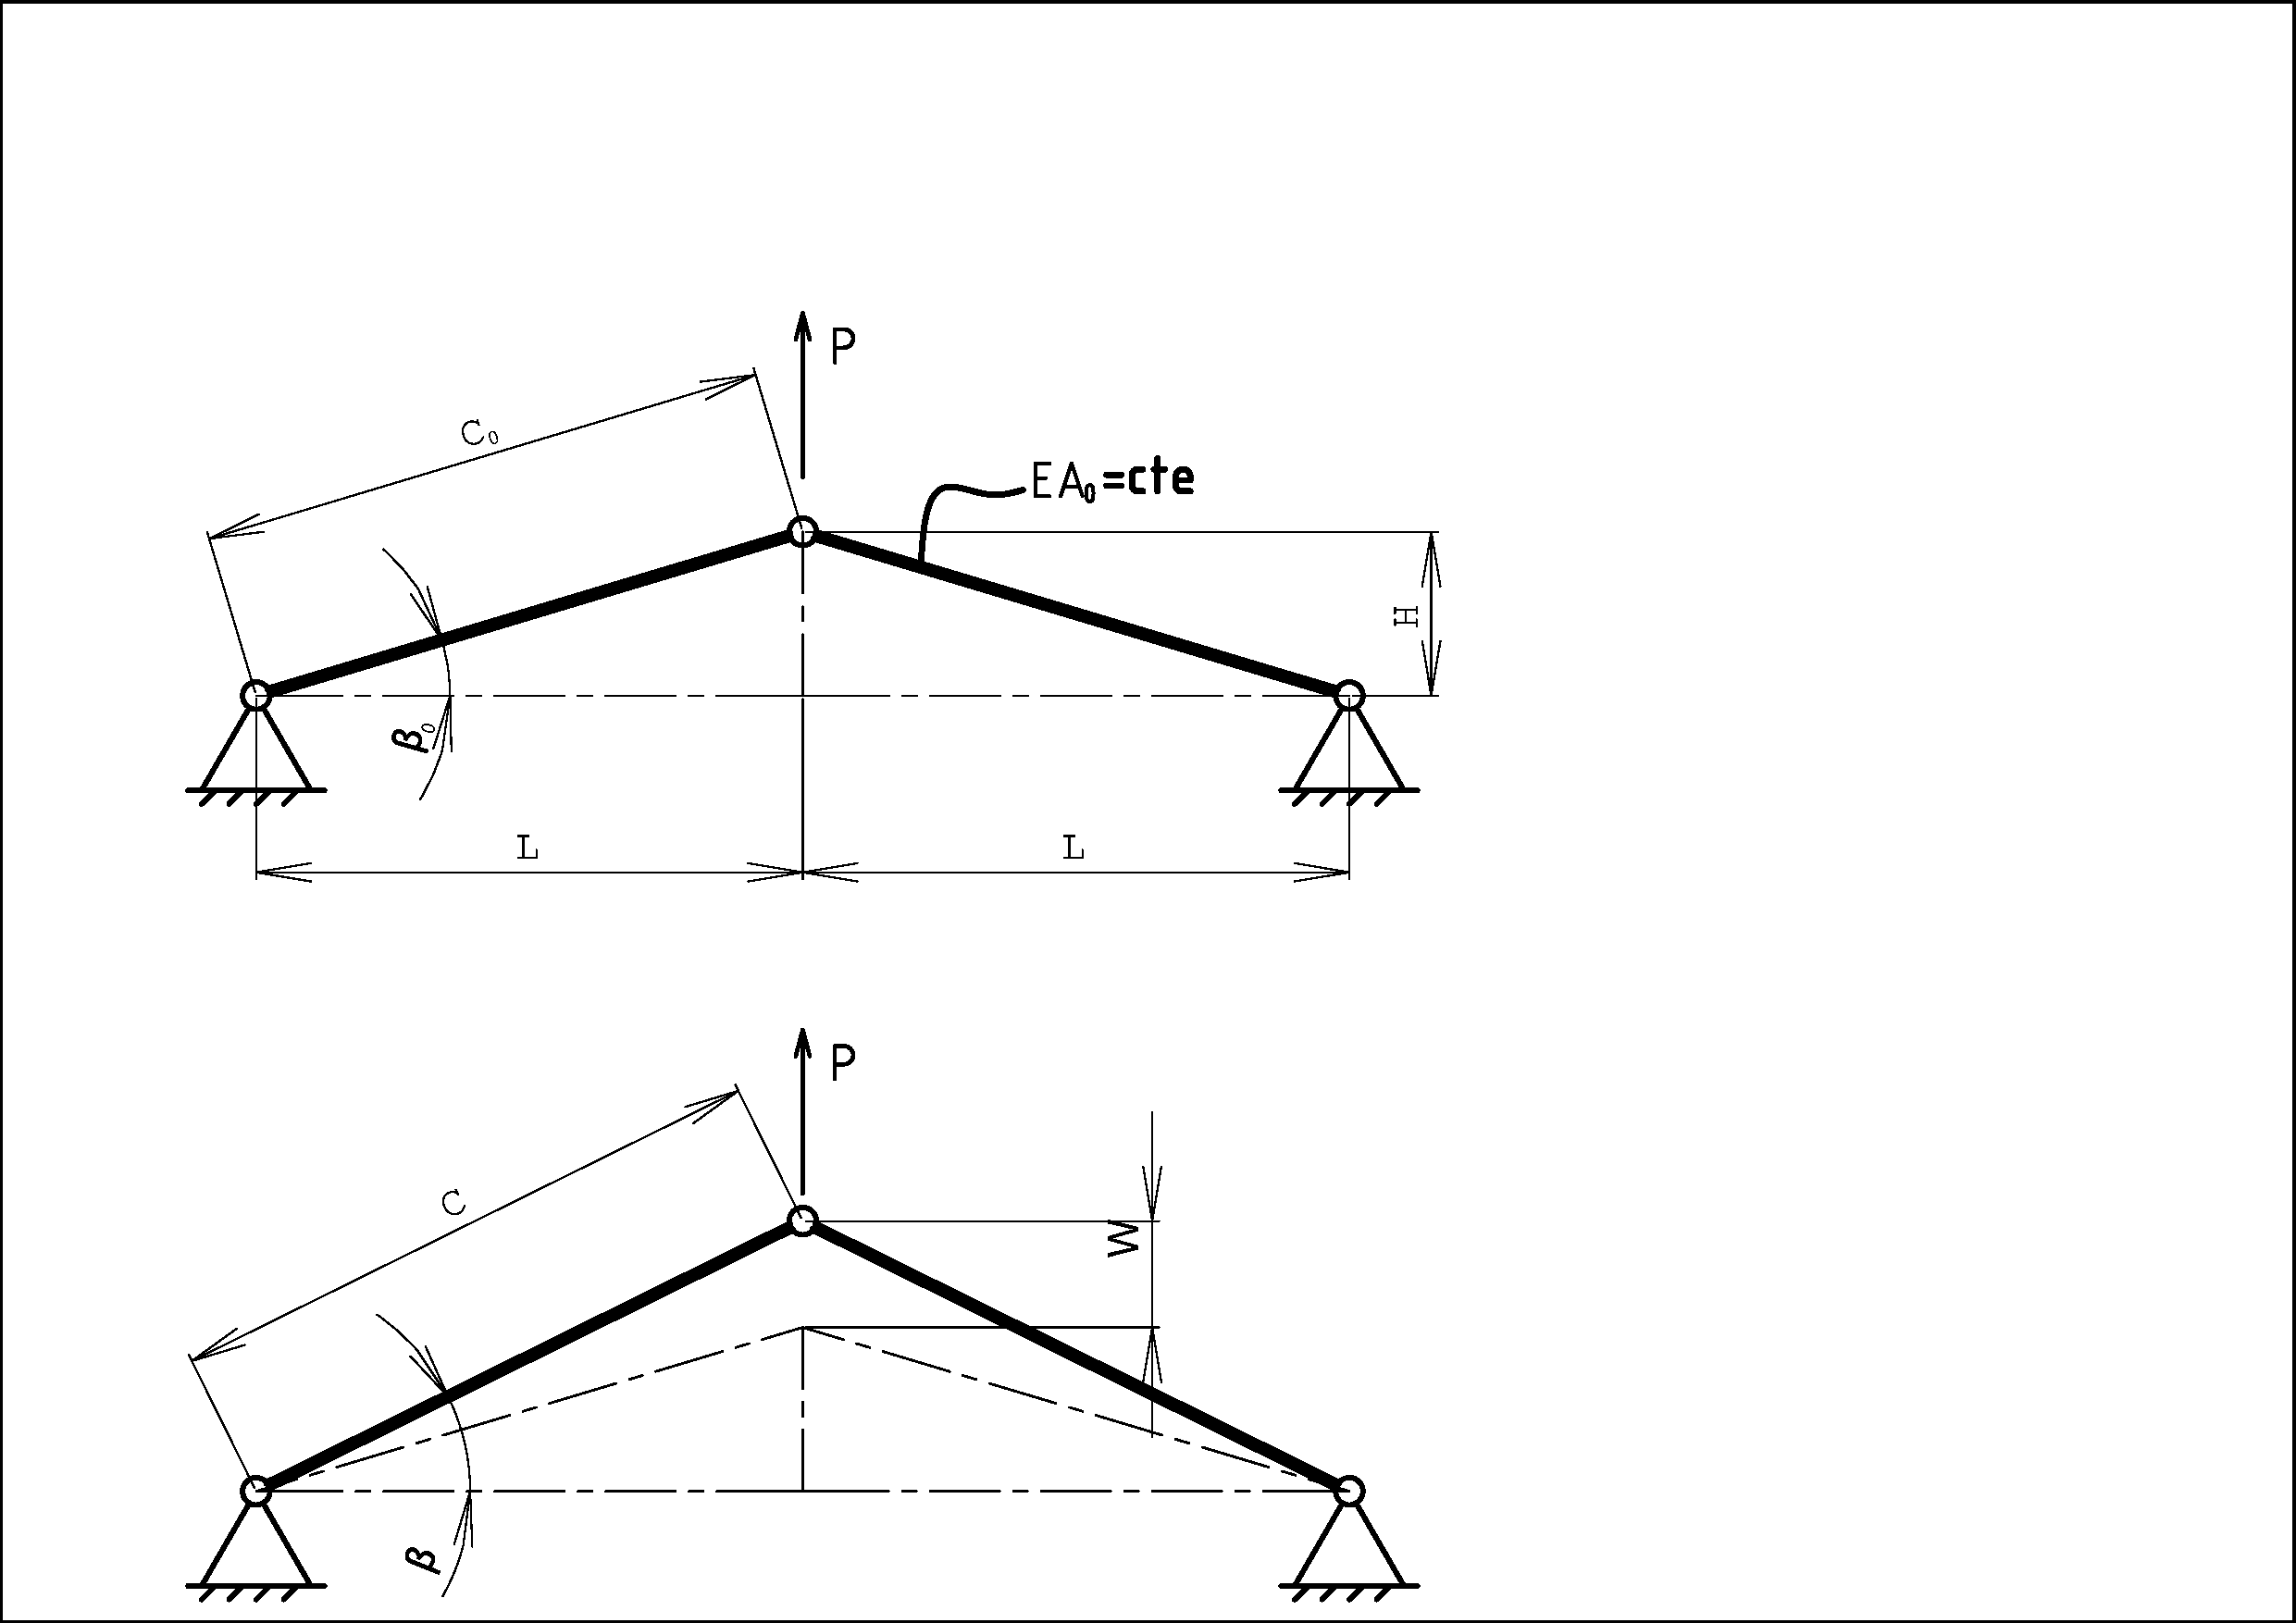
\includegraphics[
		trim=30mm 4mm 150mm 55mm,
		clip,
		width=0.6\textwidth
	]{figuras/TPs-9.pdf}
\end{figure}

$\longrightarrow$ Verificar a deformação final


% ================ Resolução TP-09 ================
\begin{textocaixa}
\hspace{10mm}





\end{textocaixa}